\documentclass[11pt]{article}

% load some asm stuff -
\usepackage{amssymb}
\usepackage{amsmath}
\usepackage{amsthm}
%\usepackage{palatino,lettrine}
\usepackage{fancyhdr}
\usepackage{epsfig}
\usepackage[round,comma,sort]{natbib}
\usepackage{simplemargins}
\usepackage{setspace}
\usepackage{boiboites}
\usepackage[margin=0pt,font=small,labelfont=bf]{caption}

\bibliographystyle{plos2009}

% Set the size
%\textwidth = 6.75 in
%\textheight = 9.75 in
%\oddsidemargin = 0.0 in
%\evensidemargin = 0.0 in
%\topmargin = 0.01 in
%\headheight = 0.0 in
%\headsep = 0.25 in
%\parskip = 0.15in
\doublespace

\setallmargins{1in}

\newtheorem{example}{Example}[section]
\newtheorem{thm}{Theorem}[section]
\newtheorem{property}{Property}[section]

\theoremstyle{definition}
\newtheorem{defn}[thm]{Definition}

\makeatletter
\renewcommand\subsection{\@startsection
	{subsection}{2}{0mm}
	{-0.05in}
	{-0.5\baselineskip}
	{\normalfont\normalsize\bfseries}}
\renewcommand\subsubsection{\@startsection
	{subsubsection}{2}{0mm}
	{-0.05in}
	{-0.5\baselineskip}
	{\normalfont\normalsize\itshape}}
\renewcommand\paragraph{\@startsection
	{paragraph}{2}{0mm}
	{-0.05in}
	{-0.5\baselineskip}
	{\normalfont\normalsize\itshape}}
\makeatother
\linespread{1.2}

\fancypagestyle{proposal}{\fancyhf{}%
	\fancyhead[RO,LE]{\thepage}%
	\fancyhead[LO,RE]{ChE 525 Simple Models of Enzyme Kinetics}%
	\renewcommand\headrulewidth{1pt}}
\pagestyle{proposal}

% Single space'd bib -
\setlength\bibsep{0pt}

\renewcommand{\rmdefault}{phv}\renewcommand{\sfdefault}{phv}

\newboxedtheorem[boxcolor=black, background=gray!5,titlebackground=orange!20,titleboxcolor = black]{color_box_example}{Example}{test}

% Change the number format in the ref list -
\renewcommand{\bibnumfmt}[1]{#1.}

% Change Figure to Fig.
\renewcommand{\figurename}{Fig.}

%Joycelyn Chan, Joshua Lequieu, Michael Paull, Chidanand Balaji, Ryan Tasseff
%Our derivation follows closely the earlier development of Fredrickson \citep{Fredrickson:1976fk}.

% Begin ...
\begin{document}

%\begin{titlepage}
{\par\centering\textbf{\Large Simple Models of Enzyme Kinetics}}
\vspace{0.2in}
{\par \centering \large{Jeffrey D. Varner$^{*}$}}
\vspace{0.05in}
{\par \centering \large{School of Chemical Engineering$^{*}$}}
{\par \centering \large{Purdue University, West Lafayette IN 47907}}
\vspace{0.1in}
{\par \centering \small{Copyright \copyright\ Jeffrey Varner 2016. All Rights Reserved.}}\\

%\end{titlepage}
\date{}
\thispagestyle{empty}

\setcounter{page}{1}

%material and energy balances around the different processes cells do. For example, understanding how the abundance of raw materials in a bioreactor influences
%cell growth, or the production of valuable protein or small molecule products requires a materials balances around the major components of the system.
%The production of valuable small molecule or protein products requires large connected intracellular reaction networks that produce or consume energy.
%Thus, to understand the operation of biochemical systems and ultimately to manipulate them for societal gain,


\section*{Introduction}
We developed material balances for nutrients, products and cells for batch, fed-batch and continuous stirred tank bioreactors where
we treated the cells as black boxes that consumed nutrients and produced products. Given our black box model of cells,
we also considered the \textit{best} way to operate bioreactors, for example, to maximize product titer or productivity
by varying process parameters, such as volumetric flow rate. However, since we treated the cells as black boxes,
we have not considered the problem of changing the \textit{intracellular} operation of cells.
To do that we need to understand how cells operate, and particularly how they process nutrients such as sugars into products.
Cells operate huge connected intracellular biochemical \textit{networks} collectively called metabolism using a special class of proteins called \textit{enzymes}.
Enzymes are proteins that catalyze the chemical reactions occurring inside simple and complex cells.
Enzymes are responsible for processing starting materials such as sugars into products of interest, waste products and eventually more cells.
Enzymes are also responsible for information processing, and biophysical functions such as transporting molecules across membranes.
Enzymes can be classified in one of six classes, based on the chemical reactions they catalyze (Fig. \ref{fig-enzyme-table}).
Just like other types of catalysts, enzyme do \textit{not} change the overall energetics of a chemical reaction, rather they lower the activation
barrier for the reaction to occur (Fig. \ref{fig-activation-barrier})

\begin{figure*}[!h]\centering
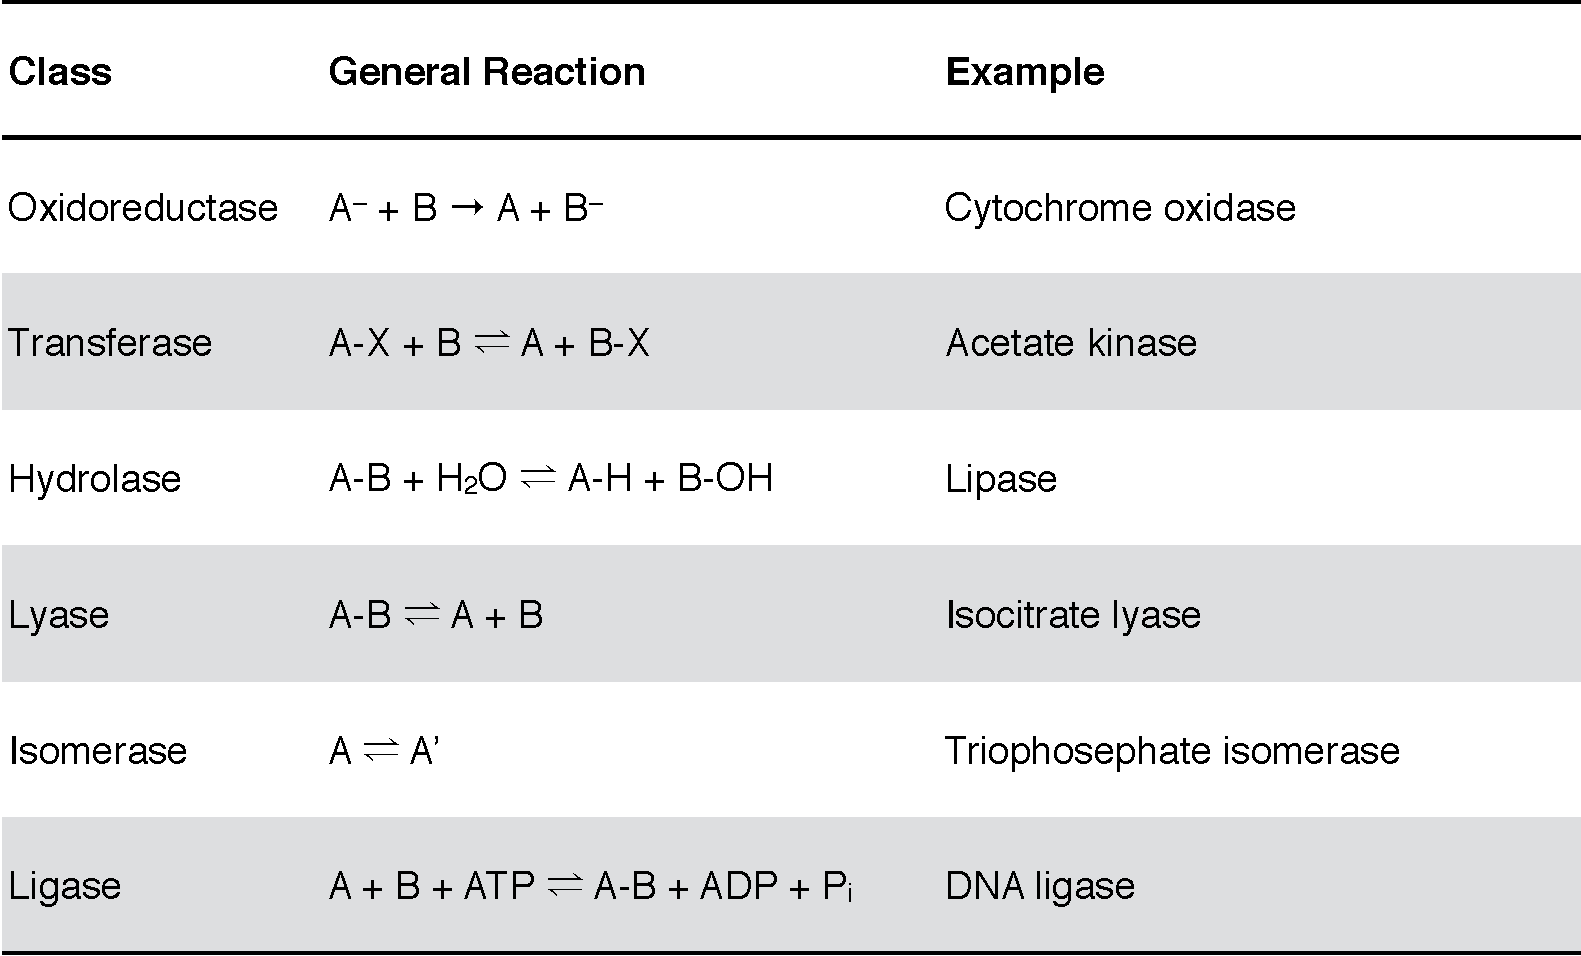
\includegraphics[width=0.9\textwidth]{./figs/Fig-EnzymeTable_v2.pdf}
\caption{Enzymes are proteins that carry out specific chemical transformations inside a cell.
There are six general classes of enzymes: Oxidoreductases, Transferases, Hydrolases, Lyases, Isomerases and Ligases.}\label{fig-enzyme-table}
\end{figure*}

\begin{figure*}[!h]\centering
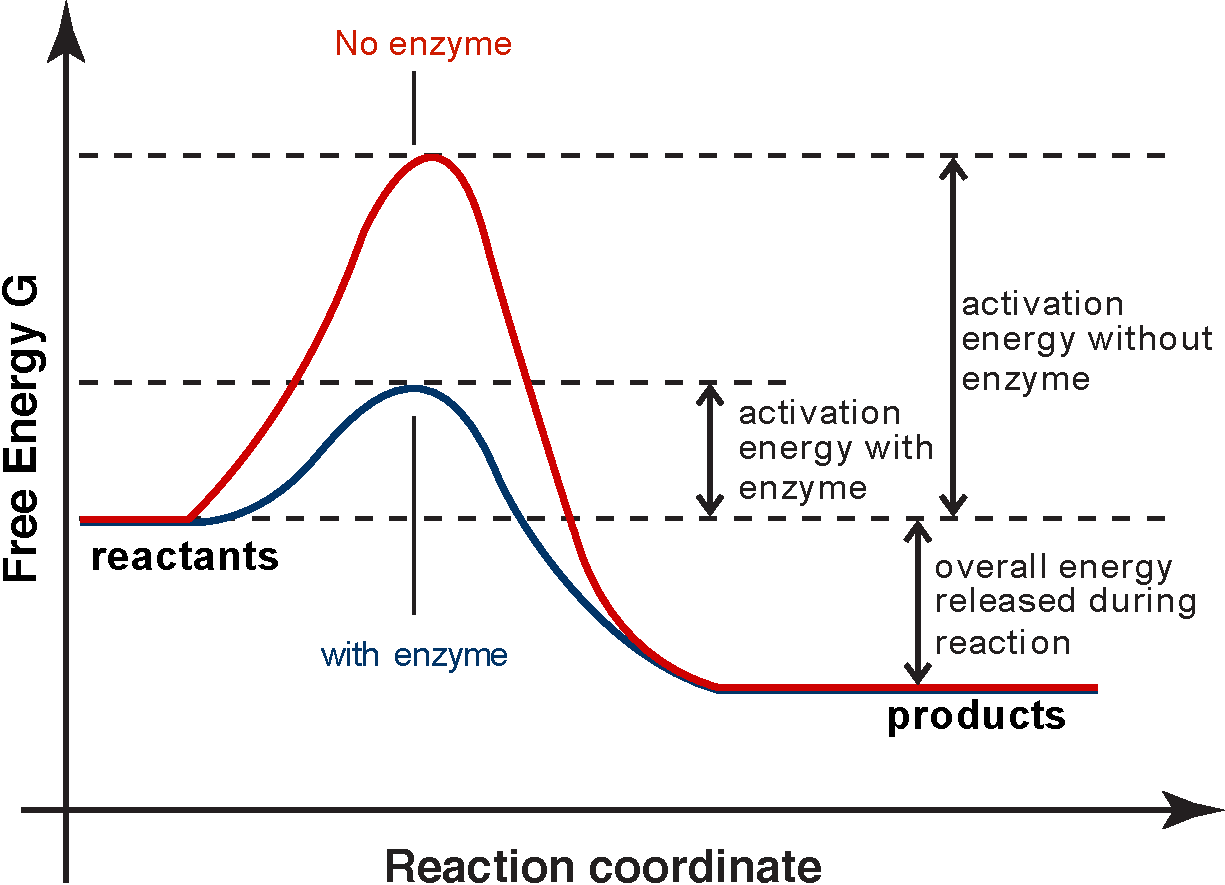
\includegraphics[width=0.8\textwidth]{./figs/Fig-ReactionCoordinate_v2.pdf}
\caption{Enzymes catalyze chemical reactions by lowering the activation energy required for the reaction to proceed.
However, enzymes do not alter the overall free energy change of the reaction. }\label{fig-activation-barrier}
\end{figure*}

\subsection*{Idealized models of enzyme kinetics.}
In general, modeling the kinetics (rate) of enzyme catalyzed reactions, for example the rate of starch degradation by $\alpha$-amylase, is a difficult problem.
However, we can gain insight into this difficult problem, and the general arguments of how to formulate the problem, by studying a simple idealized example.
Let's assume we have a well mixed test tube containing an enzyme $E$ (a protein that catalyzes chemical reactions) which converts substrate $S$ (the starting compound)
into product $P$:
\begin{equation}
S\stackrel{E}\longrightarrow{P}
\end{equation}
by an idealized \textit{lock and key} mechanism (Fig. \ref{fig-mechanism}).
\begin{figure*}[!h]\centering
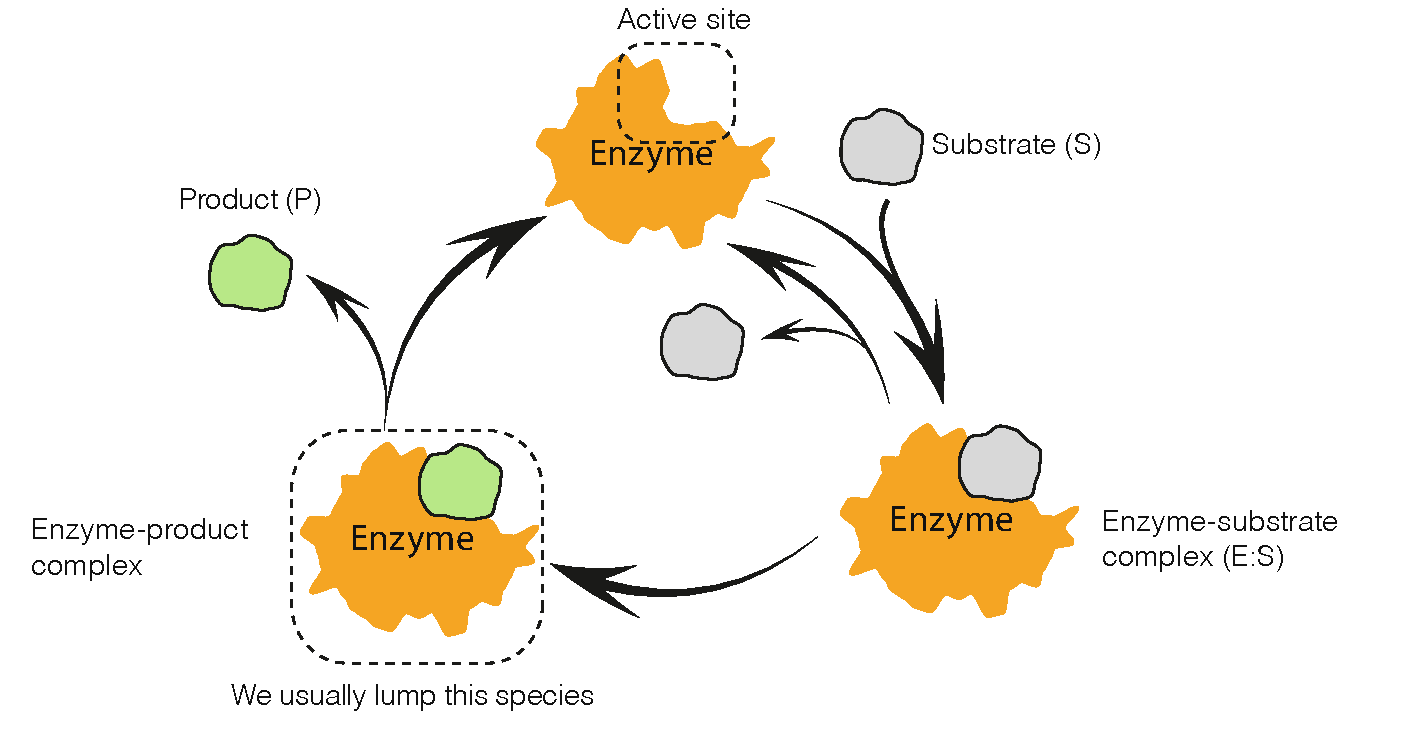
\includegraphics[width=1.0\textwidth]{./figs/EnzymeKinetics.pdf}
\caption{Schematic of the idealized \textit{lock and key} mechanism of the enzyme catalyzed conversion of substrate $S$ to product $P$ by an enzyme $E$. }\label{fig-mechanism}
\end{figure*}
The enzyme $E$ converts the substrate $S$ into the product $P$ according to the three elementary reactions:
\begin{eqnarray}
	E+S&\rightleftharpoons&{E:S}\\
	{E:S}&\longrightarrow&E+P
\end{eqnarray}
The kinetics of each elementary step can be written using \emph{mass-action} kinetics, i.e.,
\begin{eqnarray}
	r_{1} & = & k_{1}\left[E\right]\left[S\right]\\
	r_{2} & = & k_{2}\left[E:S\right]\\
	r_{3} & = & k_{3}\left[E:S\right]
\end{eqnarray}where $\left[\cdot\right]$ denotes a species concentration, and $k_{j}$ denotes the rate constant governing the $jth$ elementary reaction.
The rate $r_{1}$ describes the \emph{association} rate between the enzyme and substrate, $r_{2}$ describes the rate of \emph{dissociation} of the enzyme substrate complex and $r_{3}$ denotes the rate of \emph{chemical~conversion} of the bound substrate into product (where we assume the dissociation of the product from the enzyme is fast). Lastly, enzyme concentration must obey the relationship:
\begin{equation}\label{eqn:total-enzyme-balance-simple}
	\left[E_{T}\right] = \left[E\right] + \left[E:S\right]
\end{equation}where $\left[E_{T}\right]$ denotes the total enzyme concentration in the tube, $\left[E\right]$ denotes the \emph{free} enzyme concentration (not bound to substrate) while
$\left[E:S\right]$ denotes the enzyme substrate complex.

In order to estimate the \emph{overall} rate of enzymatic conversion ($v$) of $S$ to $P$, we need to stipulate a single rate limiting step out of the set of elementary reactions describing the conversion.
Let's assume that the rate of chemical conversion ($r_{3}$) is the \emph{slowest} step, i.e., the substrate bounces on/off the enzyme quickly with only a fraction of these binding events resulting
in a successful chemical transformation. Thus, the overall rate of S to P is then given by:
\begin{equation}\label{eqn:overall-rate-start-simple}
	v = k_{3}\left[E:S\right]
\end{equation}
Let's also assume that we already know (or can estimate) the rate constants $k_{1},k_{2}$ and $k_{3}$. When this is true, the only unknown in
Eqn. \eqref{eqn:overall-rate-start-simple} is $\left[E:S\right]$.
However, we can relate $\left[E:S\right]$ to variables we know ($E_{T}$ and at least initially $S$) through the enzyme balance,
and a second assumption called the \emph{pseudo-steady-state~assumption} for the reaction intermediate
$\left[E:S\right]$:
\begin{equation}\label{eqn:pssa-simple}
	\frac{d\left[E:S\right]}{dt} = k_{1}\left[E\right]\left[S\right] - k_{2}\left[E:S\right] - k_{3}\left[E:S\right]\simeq{0}
\end{equation}Rearranging Eqn. \eqref{eqn:pssa-simple} and solving for $\left[E:S\right]$ gives the relationship:
\begin{equation}\label{eqn:es-simple}
	\left[E:S\right]\simeq\frac{k_{1}}{k_{2}+k_{3}}\left[E\right]\left[S\right]
\end{equation}where the ratio of rate constants is defined as the Michaelis Menten saturation coefficient or $K_{M}$:
\begin{equation}
	\frac{1}{K_{M}}\equiv\frac{k_{1}}{k_{2}+k_{3}}
\end{equation}
Substituting Eqn. \eqref{eqn:es-simple} into the overall rate yields:
\begin{equation}\label{eqn:final-v-simple}
	v = k_{3}\frac{\left[E\right]\left[S\right]}{K_{M}}
\end{equation}However, in $v$ we still do not know $\left[E\right]$, the free enzyme concentration. To get $\left[E\right]$ we have to use the total enzyme balance.
Substituting Eqn. \eqref{eqn:es-simple} into the enzyme balance Eqn. \eqref{eqn:total-enzyme-balance-simple} and solving for $\left[E\right]$ yields:
\begin{equation}\label{eqn:eqn-finally-simple}
	\left[E\right] = \frac{\left[E_T\right]K_{M}}{K_{M}+\left[S\right]}
\end{equation}Lastly, we can substitute Eqn. \eqref{eqn:eqn-finally-simple} into Eqn. \eqref{eqn:final-v-simple} to arrive at the final expression for $v$:
\begin{equation}\label{eqn:mmequation-simple}
	v = V_{max}\frac{\left[S\right]}{K_{M}+\left[S\right]}
\end{equation}where $V_{max}\equiv{k_{3}}\left[E_{T}\right]$. Michaelis Menten kinetics are a type of saturation kinetics where the change in the reaction rate as a function of substrate concentration
saturates (slows down) as we increase substrate beyond a critical limiting value (Fig. \ref{fig-mm-plot}).  Similar to Monod growth kinetics, when $S\gg{K}_{M}$ the rate becomes close to $V_{max}$. Conversely,
when $S\ll{K}_{M}$ the rate appears to be linear with respect to substrate concentration.
Lastly, it is easy to show that when $K_{M}\simeq S$ the reaction rate equals $v\simeq 1/2V_{max}$.

\begin{figure*}[!h]\centering
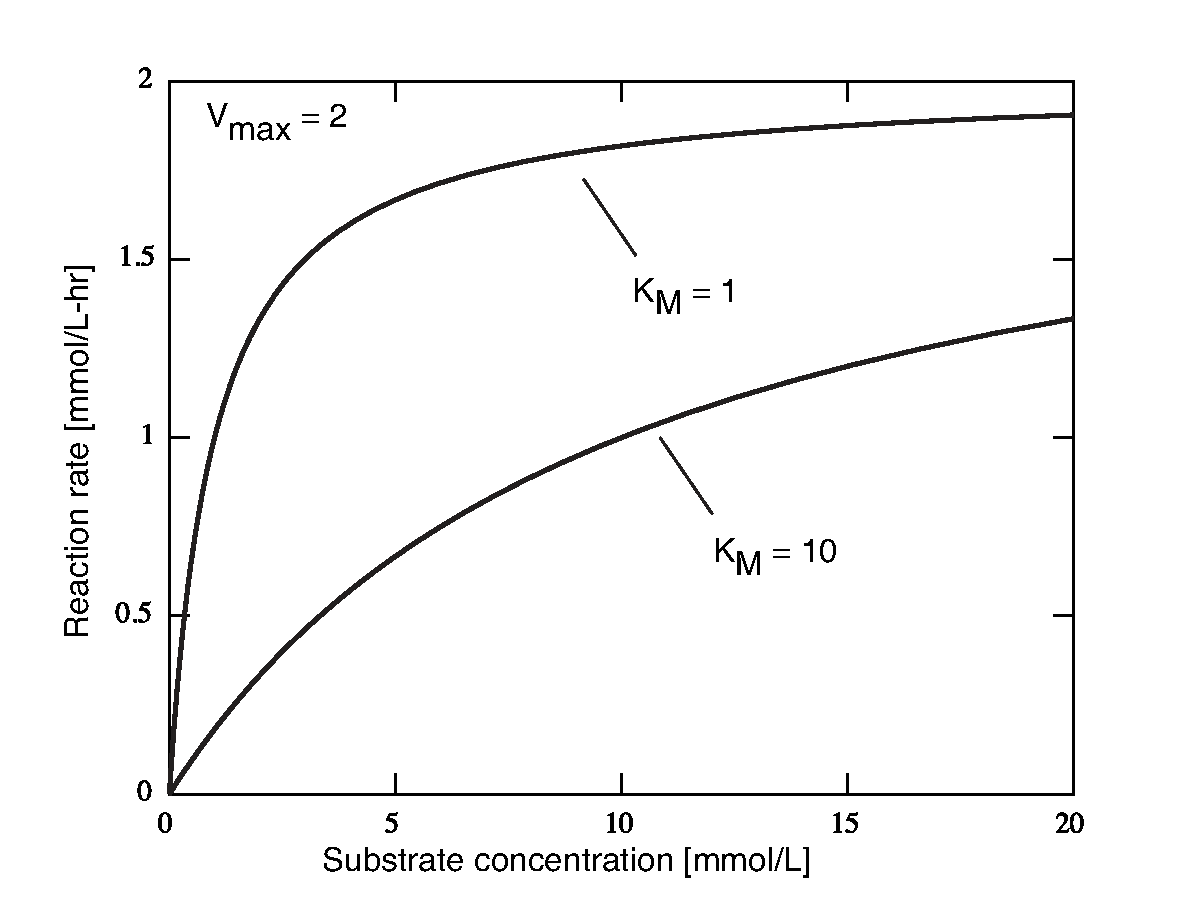
\psfig{file=figs/MMRate-Final.eps,width=0.8\textwidth}
\caption{Reaction rate versus substrate concentration for a Michaelis Menten rate form. }\label{fig-mm-plot}
\end{figure*}

\subsection*{How can we estimate $V_{max}$ and $K_{M}$ from data?}
There is no general first-principles methodology to estimate $V_{max}$ and $K_{M}$ for an arbitrary enzyme catalyzed reaction.
Thus, we must estimate these parameters from experimental measurements.
For the simple reactions we have derived we can make a \emph{Lineweaver-Burk} plot (LBP) \citep{LWBPlot}.
LBPs are a double reciprocal plot that allows us to estimate \emph{both} the $K_{M}$ and the $V_{max}$ of
an enzyme substrate pair.
Suppose we could measure the overall rate of reaction for a given substrate level.
If we invert Eqn. \eqref{eqn:mmequation-simple} and collect terms we arrive at:
\begin{equation}\label{eqn:inverse-rate}
	\frac{1}{v} = \frac{K_{M}}{V_{max}}\frac{1}{S} + \frac{1}{V_{max}}
\end{equation}Eqn. \eqref{eqn:inverse-rate} is a \emph{linear} equation; if we let $1/v$ equal the dependent variable (y-axis), and $1/S$ equal the independent variable (x-axis),
then $1/V_{max}$ is the y-intercept and
$K_{M}/V_{max}$ equals the slope (Fig \ref{fig-lwb-plot}).
\begin{figure*}[!h]\centering
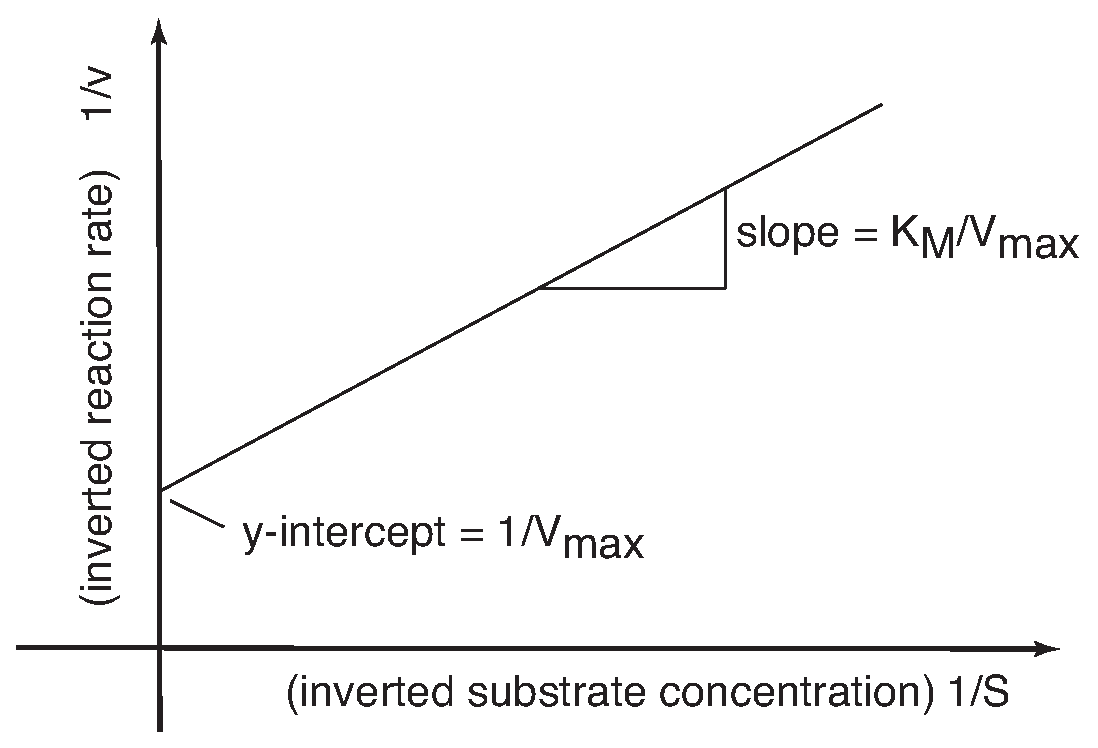
\psfig{file=figs/Lineweaver-Burke-Plot.eps,width=0.6\textwidth}
\caption{Example Lineweaver-Burk plot for a single substrate reaction in the absence of inhibitors.}\label{fig-lwb-plot}
\end{figure*}

\subsubsection*{Aside: What is the physical meaning of the $K_{M}$?}
We have already seen that the $K_{M}$ is the substrate concentration where reaction rate equals half the maximum rate.
However, $K_{M}$ also has a relationship with \textit{affinity} of an enzyme for its substrate.
The Michaelis–Menten constant $K_{M}$ is \emph{inversely} proportional to the \emph{affinity} of the enzyme for its substrate. To show this true, let's revisit our rate limiting step hypothesis.
Our development was based on the chemistry step being \emph{slow} relative the binding. When this is true, $k_{2}\gg{k_{3}}$ which implies:
\begin{equation}
	K_{M}\simeq\frac{k_{2}}{k_{1}}
\end{equation}The ratio $k_{2}/k_{1}$ is inversely related to the affinity $K_{A}$:
\begin{equation}
	K_{M}\simeq\frac{k_{2}}{k_{1}} = \frac{1}{K_{A}}
\end{equation}Thus, if an enzyme binds a substrate strongly, it has a \emph{small} $K_{M}$. Conversely, if the substrate is \emph{not} tightly held by the enzyme, then the $K_{M}$ is large.
Different $K_{M}$ values impact the reaction rate (Fig. \ref{fig-mm-plot}); as $K_{M}$ increases (the affinity decreases) more substrate is required to achieve the same reaction rate. In other words, more binding events between substrate and enzyme are required before the enzyme holds the substrate long enough for the chemistry to occur.

\subsection*{Simple models of enzyme kinetics in the presence of inhibitors.}
One of the standard laboratory (and potentially even therapeutic) tools to manipulate enzyme activity (the ability to carry out chemical function) are inhibitors.
Typically, inhibitors are small molecules that interfere with the ability of an enzyme to function in some way.
\emph{Competitive inhibitors} bind the enzyme active site (location on the enzyme where the chemical conversion of substrate to product occurs) and block the ability of the substrate to bind.
Conversely, \textit{uncompetitive} and \textit{noncompetitive} inhibitors
allow substrate binding, but modulate product formation by potentially binding regulatory sites on the enzyme (allosteric sites)
or by binding both free and bound enzymes.

\subsubsection*{Competitive inhibitors.}
Let's assume we have a well mixed test tube containing an enzyme $E$ (a protein that catalyzes chemical reactions), a competitive inhibitor $I$
and a substrate $S$ (the starting compound).
The enzyme $E$ converts the substrate $S$ into the product $P$ according to the normal elementary reactions:
\begin{eqnarray}
	E+S&\rightleftharpoons&{E:S}\\
	{E:S}&\longrightarrow&E+P\\\label{eqn-ei-binding}
	E+I&\rightleftharpoons&{E:I}
\end{eqnarray}in addition to an elementary reaction describing the reversible association of the inhibitor with the enzyme, Eqn. \eqref{eqn-ei-binding}.
Again, the kinetics of each elementary step can be written using \emph{mass-action} kinetics:
\begin{eqnarray}
	r_{1} & = & k_{1}\left[E\right]\left[S\right]\\
	r_{2} & = & k_{2}\left[E:S\right]\\
	r_{3} & = & k_{3}\left[E:S\right]\\
	r_{4} & = & k_{4}\left[E\right]\left[I\right]\\
	r_{5} & = & k_{5}\left[E:I\right]
\end{eqnarray}where $\left[\cdot\right]$ denotes a species concentration, and $k_{j}$ denotes the rate constant governing the $jth$ elementary reaction.
The rate $r_{1}$ describes the \emph{association} rate between the enzyme and substrate, $r_{2}$ describes the rate of \emph{dissociation} of the enzyme substrate complex and $r_{3}$ denotes the rate of \emph{chemical~conversion} of the bound substrate into product (where we assume the dissociation of the product from the enzyme is fast).
The last two rates ($r_{4}$ and $r_{5}$) describe the rate of association and dissociation of the enzyme-inhibitor complex.
Lastly, enzyme concentration must obey the relationship:
\begin{equation}\label{eqn:total-enzyme-balance}
	\left[E_{T}\right] = \left[E\right] + \left[E:S\right] + \left[E:I\right]
\end{equation}where $\left[E_{T}\right]$ denotes the total enzyme concentration in the tube, $\left[E\right]$ denotes the \emph{free} enzyme concentration (not bound to substrate), $\left[E:S\right]$ denotes the enzyme substrate complex and $\left[E:I\right]$ denotes the enzyme inhibitor complex.
In order to estimate the \emph{overall} rate of enzymatic conversion ($v$) of $S$ to $P$, we postulate a single rate limiting step out of the set of elementary reactions describing the conversion.
Let's assume that the rate of chemical conversion ($r_{3}$) is the \emph{slowest} step, i.e., the substrate bounces on/off the enzyme quickly with only a fraction of these binding events resulting in a successful chemical transformation. Thus, the overall rate of conversion is then given by:
\begin{equation}\label{eqn:overall-rate-start}
	v = k_{3}\left[E:S\right]
\end{equation}
Let's also assume that we already know (or can estimate) the rate constants $k_{j}$.
When this is true, the only unknown in Eqn. \eqref{eqn:overall-rate-start} is $\left[E:S\right]$.
However, we can relate $\left[E:S\right]$ to variables we know ($E_{T}$ and at least initially $S$) through the enzyme balance,
and the \emph{pseudo-steady-state~assumption} for the reaction intermediates $\left[E:S\right]$ and $\left[E:I\right]$:
\begin{eqnarray}\label{eqn:pssa}
	\frac{d\left[E:S\right]}{dt} &=& k_{1}\left[E\right]\left[S\right] - k_{2}\left[E:S\right] - k_{3}\left[E:S\right]\simeq{0}\\\label{eqn:pssa-ei}
	\frac{d\left[E:I\right]}{dt} &=& k_{4}\left[E\right]\left[I\right] - k_{5}\left[E:I\right]\simeq{0}
\end{eqnarray}
Rearranging Eqn(s). \eqref{eqn:pssa} and \eqref{eqn:pssa-ei} and solving for $\left[E:S\right]$ and $\left[E:I\right]$ gives the relationships:
\begin{eqnarray}\label{eqn:es}
	\left[E:S\right]&\simeq&\frac{k_{1}}{k_{2}+k_{3}}\left[E\right]\left[S\right]\\
	\left[E:I\right]&\simeq&\frac{k_{4}}{k_{5}}\left[E\right]\left[I\right]
\end{eqnarray}As was true without inhibitor, the ratio of rate constants in Eqn \eqref{eqn:es} is the Michaelis Menten saturation coefficient or $K_{M}$:
\begin{equation}
	\frac{1}{K_{M}}\equiv\frac{k_{1}}{k_{2}+k_{3}}
\end{equation}while the ratio of inhibitor constants:
\begin{equation}
K_{I} \equiv \frac{k_{5}}{k_{4}}
\end{equation}is defined as the equilibrium inhibition constant (units of concentration).
For \emph{tight} inhibitors $K_{I}\ll{1}$, conversely for \emph{loose} inhibitors $K_{I}\gg{1}$.
Previously, we substituted our expression for $\left[E:S\right]$ into the enzyme balance and then solved for free enzyme.
In the presence of an inhibitor we do the same thing, except we substitute both $\left[E:S\right]$ and $\left[E:I\right]$ into the enzyme balance to arrive at:
\begin{equation}\label{eqn-free-e}
	\left[E_{T}\right] = \left[E\right] + \frac{\left[E\right]\left[S\right]}{K_{M}}+\frac{\left[E\right]\left[I\right]}{K_{I}}
\end{equation}Solving Eqn. \eqref{eqn-free-e} for $\left[E\right]$ yields:
\begin{equation}\label{eqn-free-w-i}
	\left[E\right] = \frac{\left[E_{T}\right]}{1+\frac{\left[S\right]}{K_{M}}+\frac{\left[I\right]}{K_{I}}}
\end{equation}
Now that we have an expression for free enzyme, we can eliminate this unknown from our overall rate expression:
\begin{equation}\label{eqn:final-v}
	v = k_{3}\frac{\left[E\right]\left[S\right]}{K_{M}}
\end{equation}and group terms to arrive at:
\begin{equation}
	v = \frac{V_{max}\left[S\right]}{\hat{K}_{M}+\left[S\right]}
\end{equation}where $V_{max}\equiv{k_{3}}\left[E_{T}\right]$ and:
\begin{equation}
	\hat{K}_{M} \equiv K_{M}\left(1+\frac{\left[I\right]}{K_{I}}\right)
\end{equation}
Competitive inhibitors \emph{seemingly} influence the \emph{affinity} of the enzyme for its substrate (Fig. \ref{fig-mm-plot-ci}).
\begin{figure*}[!h]\centering
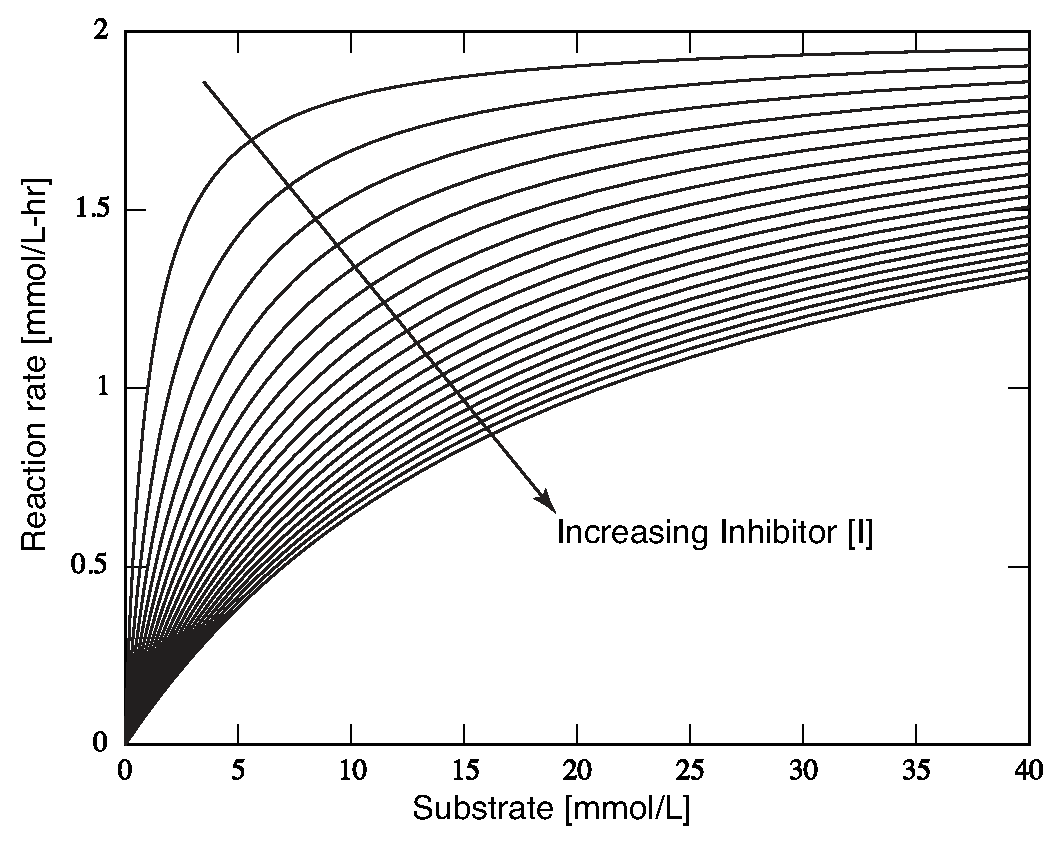
\psfig{file=figs/MMRate-CI.eps,width=0.7\textwidth}
\caption{Reaction rate versus substrate concentration for a Michaelis Menten rate form in the presence of a competitive inhibitor.}\label{fig-mm-plot-ci}
\end{figure*}

\subsubsection*{Noncompetitive inhibitors.}
The derivation for the overall enzyme catalyzed reaction rate in the presence of a noncompetitive inhibitor
follows similar arguments to the competitive case, with the exception that noncompetitive inhibitors can bind the enzyme, and the enzyme substrate complex.
Thus, the overall rate of conversion of substrate $S$ to product $P$ is modulated by the inhibitor (but not necessarily blocked).
The rate of conversion of substrate $S$ to product $P$ by enzyme $E$ in the presence of a noncompetitive inhibitor $I$ is given by:
\begin{equation}
	v = \frac{\hat{V}_{max}\left[S\right]}{K_{M}+\left[S\right]}
\end{equation}where $\hat{V}_{max}$ is given by:
\begin{equation}
	\hat{V}_{max} \equiv \frac{k_{3}\left[E_{T}\right]}{1+\frac{\left[I\right]}{K_{I}}}
\end{equation}
Noncompetitive inhibitors \emph{seemingly} influence the \emph{maximum rate} that an enzyme can convert its substrate to product (Fig. \ref{fig-mm-plot-nci}).
\begin{figure*}[!h]\centering
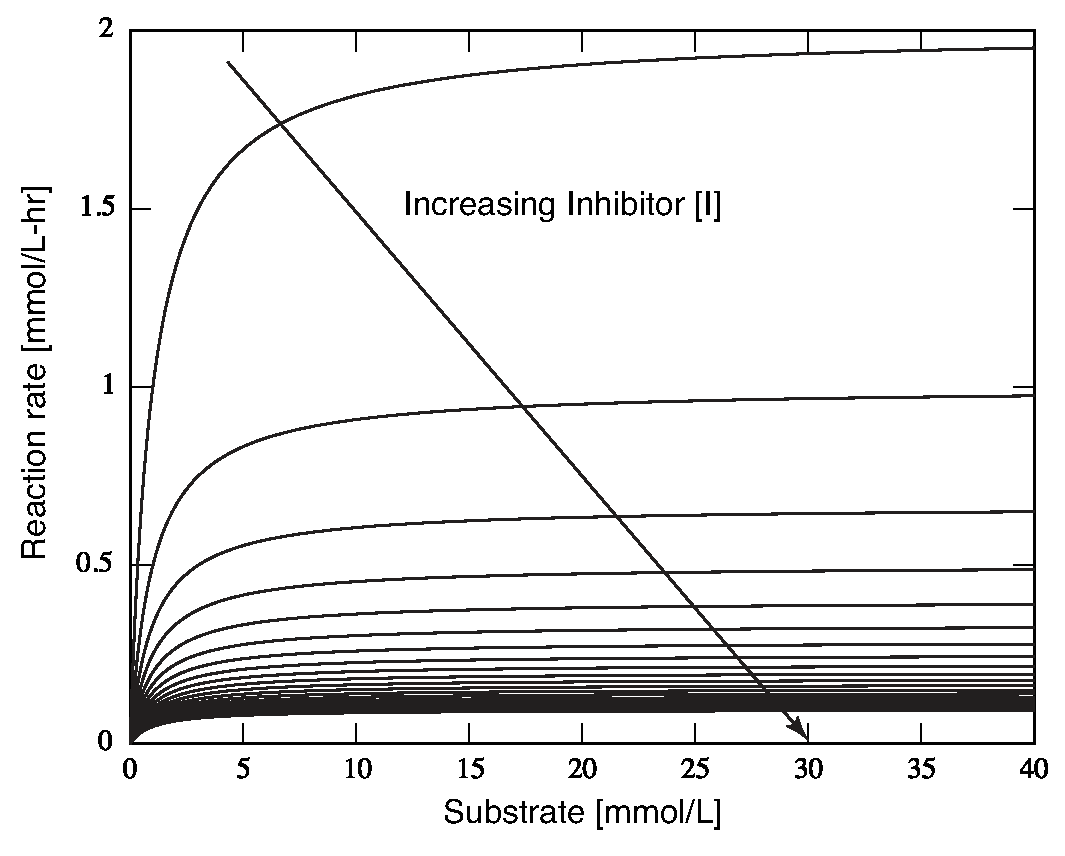
\psfig{file=figs/MMRate-NCI.eps,width=0.7\textwidth}
\caption{Reaction rate versus substrate concentration for a Michaelis Menten rate form in the presence of a noncompetitive inhibitor.}\label{fig-mm-plot-nci}
\end{figure*}

\subsubsection*{Uncompetitive inhibitors.}
Uncompetitive inhibitors exclusively bind the enzyme substrate complex, and have no affinity for the enzyme alone.
The rate of conversion of substrate $S$ to product $P$ by enzyme $E$ in the presence of a uncompetitive inhibitor $I$ is given by:
\begin{equation}
	v = \frac{\hat{V}_{max}\left[S\right]}{\hat{K}_{M}+\left[S\right]}
\end{equation}where $\hat{V}_{max}$ is given by:
\begin{equation}
	\hat{V}_{max} \equiv \frac{k_{3}\left[E_{T}\right]}{1+\frac{\left[I\right]}{K_{I}}}
\end{equation}and:
\begin{equation}
	\hat{K}_{M} = K_{M}\left({1+\frac{\left[I\right]}{K_{I}}}\right)^{-1}
\end{equation}
Uncompetitive inhibitors \emph{seemingly} decrease both the \emph{maximum rate} that an enzyme can convert its substrate to product, and the saturation constant (Fig. \ref{fig-mm-plot-nci}).
\begin{figure*}[!ht]\centering
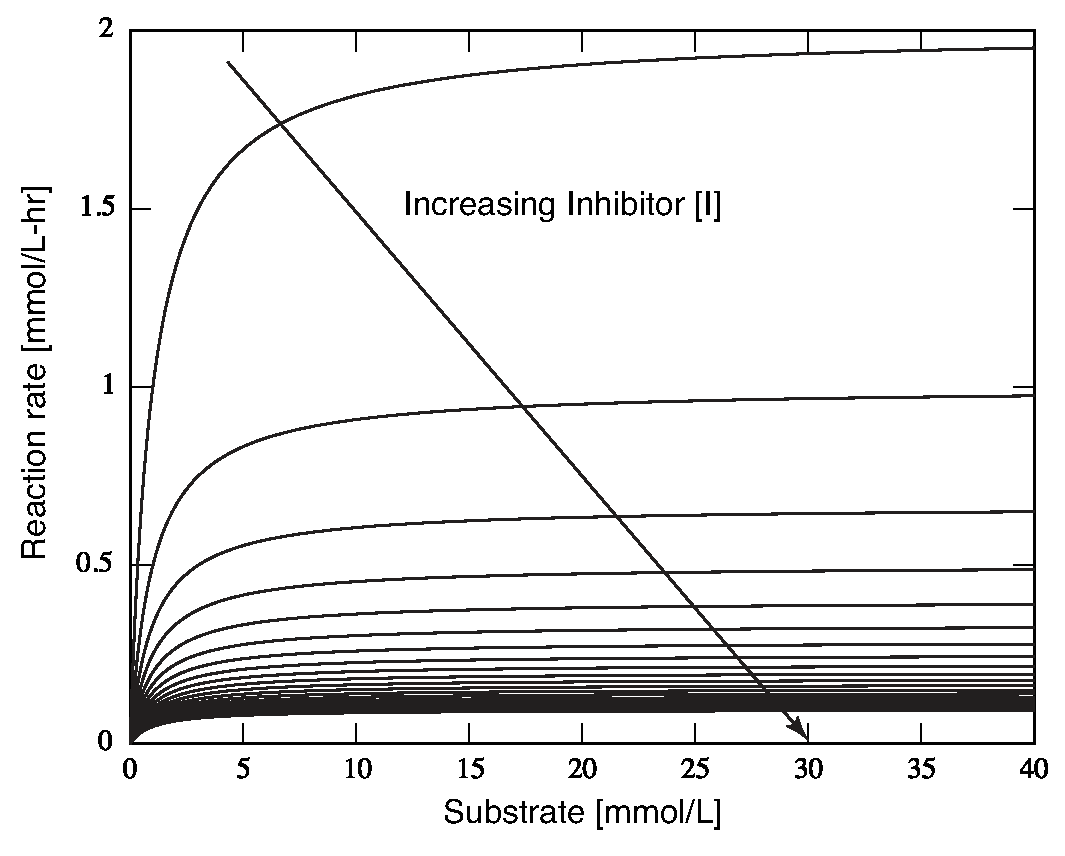
\psfig{file=figs/MMRate-NCI.eps,width=0.7\textwidth}
\caption{Reaction rate versus substrate concentration for a Michaelis Menten rate form in the presence of a noncompetitive inhibitor.}\label{fig-mm-plot-nci}
\end{figure*}

\clearpage

\bibliography{Notes}
\end{document}
